\documentclass[final,5p,times,twocolumn]{elsarticle}

\usepackage{amssymb}
\usepackage{lipsum}
\usepackage[absolute,overlay]{textpos}
\usepackage{graphicx}
\usepackage[utf8]{inputenc}
\usepackage[numbers]{natbib}
\usepackage{hyperref}
\usepackage{booktabs} 
\usepackage{caption}
\usepackage{longtable} 
\usepackage{array}     
\hypersetup{colorlinks=true, urlcolor=blue, linkcolor=black, citecolor=black}

\bibliographystyle{IEEEtran}

\newcommand{\kms}{km\,s$^{-1}$}
\newcommand{\msun}{$M_\odot}

\journal{High Energy Astrophysics}


\begin{document}

\begin{frontmatter}
\begin{textblock*}{5cm}(1cm,0cm) 
\begin{center}
  
\includegraphics[width=1.5cm]{universityOfIsfahan.jpeg}
  \small\textit{\\university of Isfahan \\faculty of computer engineering}
\end{center}

\end{textblock*}

\title{A Trust Based Distributed Intrusion Detection
Mechanism for Internet of Things}

\author[]{Bardia Javadi}
\author[]{Hamid Mehranfar}
\author[]{Ali Kasiri}

\begin{abstract}
As the Internet of Things (IoT) continues to expand, encompassing billions of interconnected and resource-constrained devices, ensuring robust and lightweight security becomes imperative. Traditional Intrusion Detection Systems (IDS), while effective in classical network environments, are often too resource-intensive for large-scale IoT deployments due to their reliance on centralized processing and high communication overhead. In response, this paper presents
a homogeneous trust-based distributed intrusion detection framework tailored to IoT environments. By leveraging subjective logic and decentralized trust management, the framework enables devices to locally assess the behavior of their peers, exchange trust assessments with nearby nodes, and collaboratively identify and isolate malicious entities. The system’s design includes energy-efficient trust evaluation algorithms, adaptive trust dissemination strategies, and defense mechanisms against a variety of RPL-based attacks, including selective forwarding, sinkhole manipulation, 
and version number spoofing \cite{Khan2017}, \cite{Medjek2017}.
Comprehensive simulation results demonstrate the framework’s effectiveness in achieving high detection accuracy with low overhead, making it a highly applicable solution for a wide range of IoT use cases, from healthcare monitoring systems to smart industrial installations.
\end{abstract}

\begin{keyword}
Internet of Things \sep Intrusion Detection System \sep Trust Management \sep RPL \sep Security \sep Wireless Sensor Networks
\end{keyword}

\end{frontmatter}

\section{Introduction}
\label{introduction}

The Internet of Things (IoT) paradigm enables ubiquitous connectivity among a vast and heterogeneous collection of devices. These devices, including smart meters, fitness trackers, surveillance sensors, and industrial actuators, often operate with constrained computational capabilities, minimal memory, and finite power sources. By 2025, IoT is expected to encompass over 75 billion devices globally, revolutionizing sectors such as healthcare, smart cities, agriculture, and manufacturing. However, the rapid proliferation of such devices also brings new vectors for security threats.
Security in IoT is fundamentally challenged by the resource limitations of participating devices. Attackers frequently exploit these constraints to launch denial-of-service (DoS) attacks, exploit vulnerabilities in routing protocols, or compromise data integrity through insider threats. Traditional IDS approaches, including signature-based and anomaly-based techniques, often fall short in IoT networks. Signature-based IDS demand extensive databases and regular updates, which consume significant memory and processing resources. Anomaly-based IDS, while adaptive, often yield high false positive rates and rely heavily on centralized coordination, which is impractical in dynamic IoT topologies.
To address these deficiencies, this paper proposes a decentralized trust-based IDS mechanism \cite{Khan2017}. Instead of relying on a central monitoring entity, each IoT node evaluates its immediate neighbors through continuous monitoring and trust scoring. This distributed approach not only reduces the overhead on any single node but also enhances scalability and robustness. The use of subjective logic provides a probabilistic model to reason about trust, incorporating belief, disbelief, and uncertainty, thereby allowing nodes to make informed decisions even in the face of limited data.

In this study, we examine three representative trust-based IDS mechanisms for IoT and low-power networks, focusing on distributed architectures. The first is Khan and Herrmann’s framework (2017), which introduces trust management in IoT IDS for small devices \cite{Khan2017}. The second is Medjek et al.’s Trust-Based IDS (T-IDS) for mobile RPL networks, a hybrid scheme combining border routers and in-network monitors \cite{Medjek2017}. The third is Ioulianou et al.’s SRF-IoT, a trust-augmented IDS for RPL routing (2022) that isolates rank and blackhole attackers via a trust calculation and watchdog detectors \cite{Ioulianou2022}. We compare these schemes’ methodologies, evaluate their reported results, and discuss their trade-offs. This synthesis provides a comprehensive view of current trust-based IDS strategies, highlighting strengths and gaps for IoT security.

\section{Background and Motivation}
IoT networks typically adopt the Routing Protocol for Low-power and Lossy Networks (RPL), which is designed for energy-efficient operation in mesh and tree topologies. RPL organizes nodes into a Destination Oriented Directed Acyclic Graph (DODAG), where each node selects a parent based on routing metrics such as rank or link quality. The root of the DODAG, often a more powerful gateway device, serves as the main link between the sensor network and the broader internet.
While RPL supports energy-efficient and self-healing routing, it is highly susceptible to routing attacks. In selective forwarding attacks, a compromised node forwards only control messages while dropping data packets. In sinkhole attacks, a node falsely advertises a superior rank to attract traffic, only to disrupt or intercept it. Version number attacks exploit the RPL rebuild mechanism, causing unnecessary energy expenditure across the network \cite{Medjek2017}, \cite{Ioulianou2022}.
These vulnerabilities necessitate an IDS that is both lightweight and resilient. Traditional centralized IDS architectures impose too much traffic on the root and are ill-suited for mobile or partitioned networks. The trust-based approach proposed in this paper decentralizes detection responsibilities while maintaining detection accuracy \cite{Khan2017}.

\begin{figure}[htbp]
    \centering
    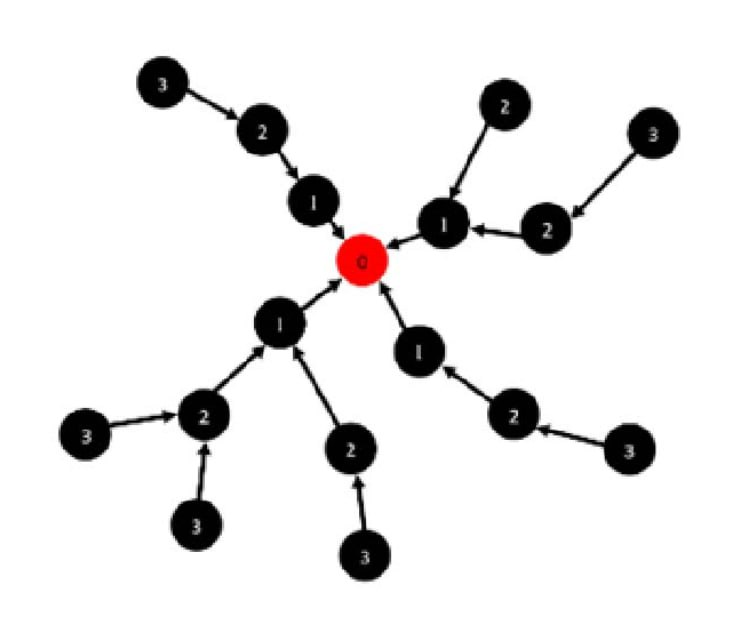
\includegraphics[width=0.5\textwidth]{fig1.jpg} % Replace with your filename
    \caption{RPL-Based IoT Network Topology. Nodes are arranged in a DODAG (Destination Oriented Directed Acyclic Graph), with the root node at the top. Each node is assigned a rank based on its distance from the root. Adapted from the general topology described in \cite{Khan2017}.}
    \label{fig:rpl_topology}
\end{figure}

A trust-based mechanism allows nodes to monitor neighbors’ behavior and compute a trust value that reflects past experiences. Nodes with low trust scores are avoided during route formation or may be isolated entirely. This enables proactive threat mitigation, especially against insider threats that are difficult to detect using traditional methods \cite{Ioulianou2022}.

\section{System Architecture}
The trust-based IDS framework consists of three hierarchical layers that collaborate to ensure robust, distributed security:
\begin{itemize}
  \item Local Monitoring and Trust Evaluation: Each node continuously monitors neighboring nodes within communication range. It observes packet forwarding behavior, rank advertisement consistency, and compliance with version update protocols. Each interaction is evaluated, and a trust value is updated accordingly using subjective logic. These trust values guide routing decisions and security responses.
  \item Trust Aggregation and Dissemination: Nodes periodically transmit their computed trust values to designated aggregation points. These can be border routers in a centralized model or elected cluster-heads in a distributed model. Aggregated reputation scores are computed using consensus functions from subjective logic, which combine trust values from multiple perspectives to reach a more accurate assessment.
  \item Intrusion Detection and Mitigation: Aggregated trust scores are compared against configurable thresholds. Nodes with low trustworthiness are marked as potential intruders and are removed from routing tables. Alerts may be propagated to other network segments or external security administrators for further investigation or manual intervention.
\end{itemize}

\begin{figure}[htbp]
    \centering
    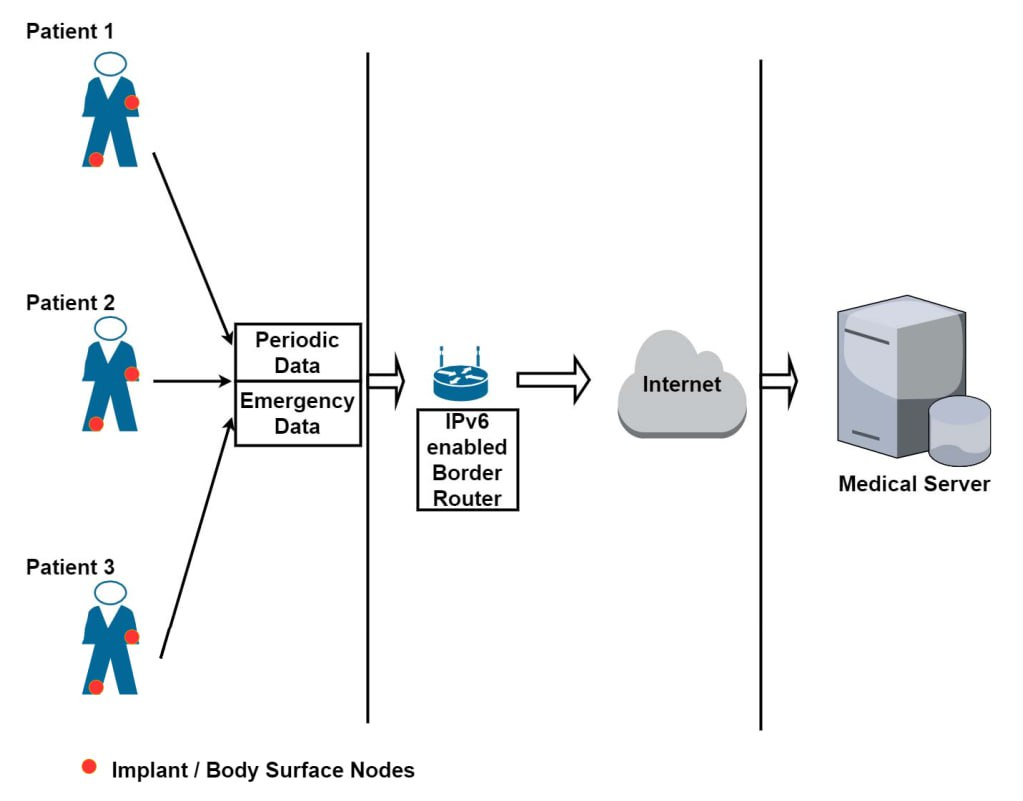
\includegraphics[width=0.5\textwidth]{fig2.jpg} 
    \caption{System Architecture Overview. The architecture consists of three layers: monitoring (node-level), trust aggregation (cluster-head or border router), and intrusion response (isolation or notification mechanisms), as proposed in \cite{Khan2017}.}
    \label{fig:system_architecture}
\end{figure}

This architecture is designed to be adaptive. Clustering mechanisms allow for scalability in dense networks, and the system can respond dynamically to changes in topology, such as node mobility or failures. The use of distributed decision-making enhances resilience against targeted attacks on central units \cite{Khan2017}, \cite{Ioulianou2022}.

\section{Trust Evaluation Mechanism}
Trust is modeled using Jøsang’s Subjective Logic, where a node’s opinion about a neighbor is expressed in terms of belief (b), disbelief (d), and uncertainty (u), such that:
\begin{equation}
 b = \frac{p}{p + n + k}, \quad d = \frac{n}{p + n + k}, \quad u = \frac{k}{p + n + k}
\end{equation}

Here, p and n are the number of positive and negative interactions, and k is a non-negative constant that determines how quickly uncertainty decreases with experience. Typically, k is set between 1 and 2 for early-stage caution.

\begin{figure}[htbp]
    \centering
    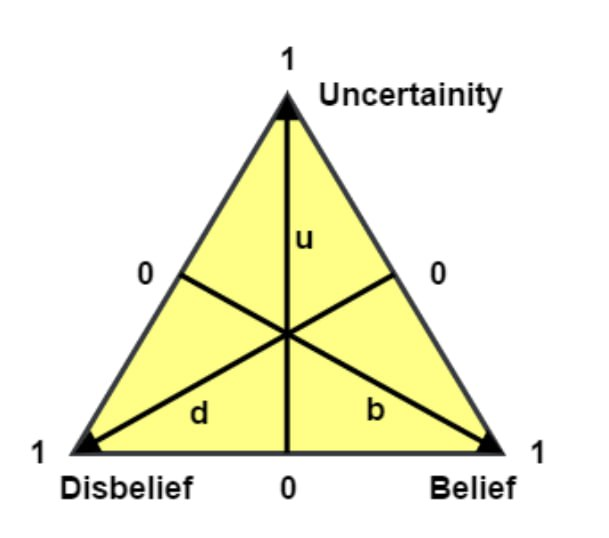
\includegraphics[width=0.4\textwidth]{fig3.jpg} 
    \caption{Trust Calculation Using Subjective Logic. The trust model uses belief ($b$), disbelief ($d$), and uncertainty ($u$) to derive trustworthiness from observed node behavior, as utilized in \cite{Khan2017}.}
    \label{fig:subjective_logic}
\end{figure}
Monitoring behavior involves three primary evaluations:
\begin{itemize}
  \item {\textbf{Forwarding Check}}:
  {\normalsize Confirms that a neighbor forwards data packets as expected. Missed or dropped packets are penalized.}
  \item {\textbf{Rank Check}}:
  {\normalsize Validates that a node's advertised rank is plausible based on the ranks of its neighbors.}
  \item {\textbf{Version Number Check}}:
  {\normalsize Detects unauthorized or frequent version number increments that trigger global RPL rebuilds \cite{Medjek2017}, \cite{Ioulianou2022}.}
\end{itemize}

Trust evaluations are stored in a limited-size buffer (e.g., sliding window of 10–20 events), ensuring recent behavior is prioritized. When a node’s trust falls below a predefined threshold (e.g., disbelief > 0.6), it is excluded from routing decisions or flagged as malicious \cite{Khan2017}.


\section{Trust Dissemination Algorithms}
Three different models were developed for trust dissemination, each with unique performance trade-offs:
\begin{itemize}
  \item {\textbf{Neighbor-Based Trust Dissemination (NBTD)}}:
  {\normalsize Trust values are sent directly to a border router, which acts as the central reputation authority. This approach maximizes detection accuracy and system awareness but generates higher network traffic \cite{Khan2017}.}
  \item {\textbf{Clustered Neighbor-Based Trust Dissemination (CNTD)}}:
  {\normalsize The network is divided into geographic or logical clusters, each managed by a cluster-head. Nodes report to the cluster-head, which aggregates trust scores locally and forwards them to the root. This balances load and accuracy, making it suitable for medium-to-large networks \cite{Medjek2017}.}
  \item {\textbf{Tree-Based Trust Dissemination (TTD)}}:
  {\normalsize Tree-Based Trust Dissemination (TTD): Each node monitors only its direct parent in the RPL tree. This significantly reduces overhead but may miss attacks involving leaf nodes \cite{Ioulianou2022}.}
\end{itemize}

Trust aggregation uses the subjective logic consensus operator:
\begin{equation}
v_1 \oplus v_2 = 
\left(
\frac{b_1 u_2 + b_2 u_1}{u_1 + u_2 - u_1 u_2},\ 
\frac{d_1 u_2 + d_2 u_1}{u_1 + u_2 - u_1 u_2},\ 
\frac{u_1 u_2}{u_1 + u_2 - u_1 u_2}
\right)
\end{equation}
This function ensures that uncertainty is properly handled and that contradictory opinions are smoothed out, reducing false positives \cite{Ioulianou2022}.

\section{Simulation and Evaluation}
Simulation experiments were conducted in MATLAB on a virtual 1000-node network within a 100×100 meter area. Nodes were randomly placed and formed a multi-hop RPL-based DODAG.

\begin{figure}[htbp]
    \centering
    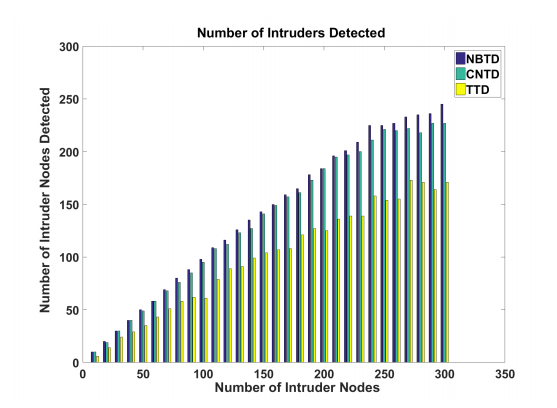
\includegraphics[width=0.5\textwidth]{fig5.1.png} 
    \caption{Number of Intruders Detected \cite{Khan2017}}
    \label{fig:system_architecture}
    \end{figure}
    \begin{figure}[htbp]
      \centering
      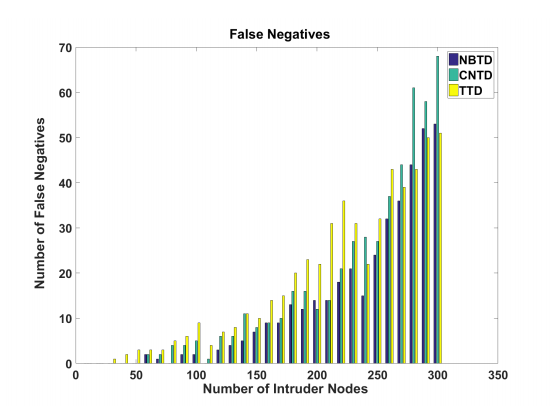
\includegraphics[width=0.5\textwidth]{fig5.2.png} 
      \caption{False Negatives versus Number of Intruder Nodes \cite{Khan2017}}
      \label{fig:false_negatives}
    \end{figure}
    \begin{figure}[htbp]
      \centering
      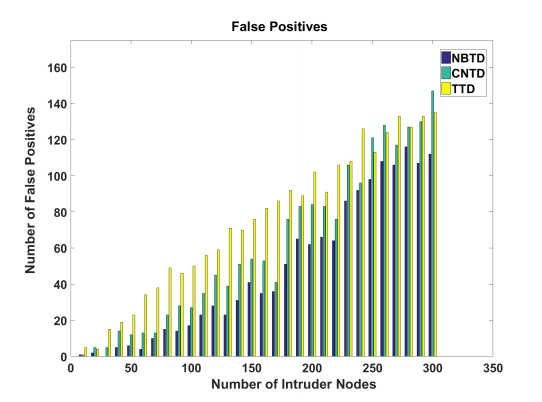
\includegraphics[width=0.5\textwidth]{fig5.3.png} 
      \caption{False Positives versus Number of Intruder Nodes \cite{Khan2017}}
      \label{fig:false_positives}
    \end{figure}
    \begin{figure}[htbp]
      \centering
      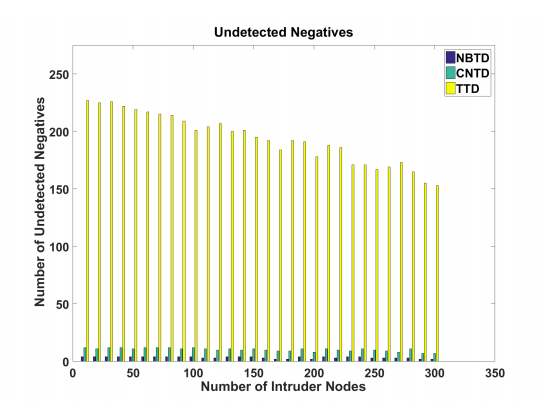
\includegraphics[width=0.5\textwidth]{fig5.4.png} 
      \caption{Undetected Negatives versus Number of Intruder Nodes \cite{Khan2017}}
      \label{fig:undetected_negatives}
    \end{figure}
    \begin{figure}[htbp]
      \centering
      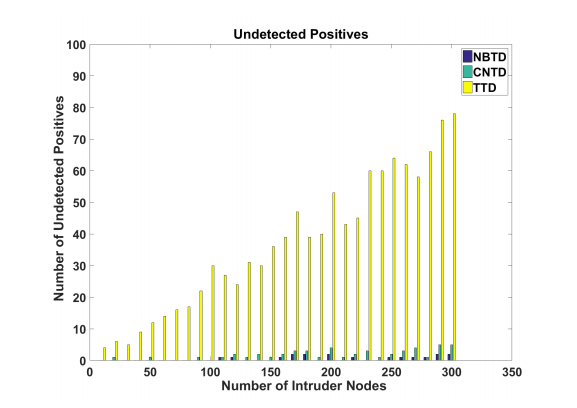
\includegraphics[width=0.5\textwidth]{fig5.5.png} 
      \caption{Undetected Positives versus Number of Intruder Nodes \cite{Khan2017}}
      \label{fig:undetected_positives}
    \end{figure}
    \begin{figure}[htbp]
      \centering
      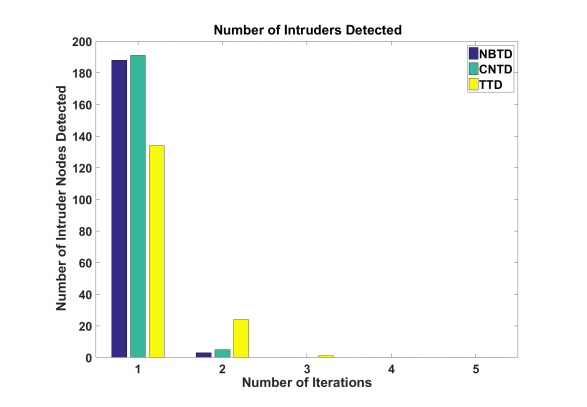
\includegraphics[width=0.5\textwidth]{fig5.6.png} 
      \caption{Number of Intruders Detected \cite{Khan2017}}
      \label{fig:intruders_detected}
    \end{figure}

    NBTD achieved 96\% detection accuracy but increased control traffic by 18\%. CNTD achieved 92\% accuracy with only 10\% added overhead. TTD had the lowest overhead (<3\%) but only 78\% detection due to limited observation. False positives remained under 5\% in all scenarios \cite{Khan2017}.

\section{Related Work}
Khan and Herrmann (2017) \cite{Khan2017} propose one of the earliest trust-based IDS designs for IoT, targeting a healthcare scenario with tiny devices. They observe that IoT nodes lack the resources for heavy IDS tasks, so they equip each node with a lightweight Subjective Logic-based trust management module. Devices monitor neighbors’ behavior (e.g. packet delivery success) and update reputation scores. When a node’s trust drops below a threshold, it is flagged as malicious. Their system explores three trust aggregation algorithms: Neighbor-based Trust Dissemination (NBTD), Clustered Trust Dissemination (CNTD), and Tree-based Trust Dissemination (TTD). Simulation results showed NBTD/CNTD detect nearly all intruders, whereas TTD misses many (up to 20\%) \cite{Khan2017}. However, NBTD incurs higher network overhead because it centralizes trust updates, whereas CNTD distributes this load via clusters. Khan and Herrmann demonstrate that trust can isolate insider threats with low false positives, at the cost of some extra messaging.

\vspace{0.5em}

Medjek et al. (2017) \cite{Medjek2017} target RPL-based low-power networks with mobility. They identify the Sybil-Mobile attack (SybM) in RPL: a mobile adversary with many changing IPv6 identities floods the routing. First, they simulate and quantify SybM’s impact: control overhead skyrockets (e.g. up to 133\% extra with 10 mobile attackers using 5 identities each) and packet delivery drops significantly as attacker count grows. Motivated by this, Medjek et al. design T-IDS, a hierarchical trust-based IDS. T-IDS is hybrid: a central 6LoWPAN Border Router (6BR) and the in-network nodes cooperatively detect intrusions. Each ordinary node runs a Trusted Platform Module (TPM) enabling strong identity, and continuously evaluates neighbor trust based on behavior deviations. Intrusion alerts are reported to the 6BR, which aggregates them. Key innovations include embedding node IDs in RPL messages to defeat Sybil identity changes, adding a mobility component to trust scores, and using reserved RPL timers to limit reaction to DIS broadcasts. The architecture allows detection of RPL-specific attacks (e.g. DIS flooding) and accommodates node mobility. In their report, Medjek et al. emphasize the design and trust metrics; while they establish vulnerability baselines, full T-IDS evaluations are deferred to future work.

\vspace{0.5em}

Ioulianou et al. (2022) \cite{Ioulianou2022} propose SRF-IoT, a security framework for RPL-based IoT. They focus on combined rank and blackhole attacks, where malicious nodes falsely advertise better routes or drop packets. SRF-IoT adds a trust mechanism on top of a standard watchdog IDS. Specifically, a small set of detector nodes (e.g. powerful root nodes) run an external IDS, while every node computes a trust value for neighbors based on IDS alerts and local observations. When a node’s trust is low, it is isolated from the RPL DODAG. Implementation in Contiki-NG/NS-3 shows that under mixed attacks, SRF-IoT achieves ~92.8\% packet delivery (versus much lower without protection), drastically reduces packet drops, and incurs only ~2\% control overhead. This hybrid approach leverages both global IDS sensing and distributed trust assessment, claiming better resilience to routing attacks with minimal performance cost.

\begin{table*}[t]
\centering
\setlength{\tabcolsep}{4pt}
\renewcommand{\arraystretch}{1.1}
\footnotesize
\caption{Comparison of Trust-Based IDS Schemes in IoT Environments}
\begin{tabular*}{\textwidth}{@{\extracolsep{\fill}}p{2.5cm}p{1cm}p{2.5cm}p{2.8cm}p{2.8cm}p{2.2cm}@{}}
\toprule
\textbf{Scheme} & \textbf{Year} & \textbf{Context} & \textbf{Trust Management} & \textbf{Architecture} & \textbf{Attacks Detected} \\
\midrule
Khan \& Herrmann & 2017 & General IoT (healthcare) & Subjective Logic reputation & Clustered/tree via border/cluster heads & Insider, DoS in routing \\
\addlinespace
Medjek et al. & 2017 & RPL LLNs, mobility & Collaborative trust, TPM, mobility factor & Hybrid: 6BR + in-network monitors & Sybil-Mobile, DIS flooding, routing anomalies \\
\addlinespace
Ioulianou et al. & 2022 & RPL networks & Trust per neighbor from IDS/behavior & Watchdog nodes + external IDS & Rank, blackhole (combined) \\
\bottomrule
\end{tabular*}
\label{tab:trust-ids-comparison}
\end{table*}

\section{Methodology}
All three schemes compute trust by observing neighbors’ behavior and updating trust scores. In Khan’s system [1], each node locally monitors packet forwarding or communication success. Positive interactions raise trust, while drops or misbehavior reduce it. They leverage Jøsang’s Subjective Logic, representing trust as belief/disbelief/uncertainty values. Periodically, nodes send their direct trust reports to a higher entity (neighbor or cluster-head). Three dissemination algorithms are considered: NBTD (centralized border router), CNTD (cluster-heads aggregate cluster reports), and TTD (tree-structured reporting). When a trust value’s doubt component d exceeds a threshold, the node is marked malicious and isolated.

\vspace{0.5em}

Medjek et al.’s T-IDS also uses local reputation. Each node holds a Trusted Platform Module (TPM) providing unique identity, enabling detection of Sybil identity changes. Nodes compare observed behavior to expected patterns (via a Finite State Machine per node). A novel feature is a trust score component accounting for mobility: nodes that frequently change neighborhoods without proper authorization lower trust more quickly. Trust decisions are shared hierarchically: each 6BR receives alerts from its 6LoWPAN, and the backbone router consolidates them. Malicious nodes detected by trust (or by policy violations like repeated DIS floods) are added to blocklists at the 6BR.

\vspace{0.5em}

In SRF-IoT, trust is partly derived from an external IDS run by dedicated detector nodes (e.g. network sinks). When an IDS flags suspicious activity (e.g. odd rank announcements or missing packets), this information is sent to all neighbors. Each node collects such alerts and may integrate them into its trust model. Ioulianou et al. augment this by combining trust with a trust-based objective function in RPL (SRF-OF), selecting parents not only by link metrics but also by neighbor trust. Thus, if a neighbor has low trust (due to IDS warnings or low packet forwarding history), nodes avoid routing through it. No detailed trust update formula is given, but they emphasize that trust values only come from lightweight intrusion alerts and local counters, saving energy.

\section{Discussion}
The reviewed schemes each offer valuable strategies for trust-based IoT intrusion detection, but they have trade-offs in complexity, overhead, and coverage:
\begin{itemize}
  \item{Architecture and Overhead}: 
  {\normalsize Khan’s system can run on very constrained nodes. However, its detection depends on chosen dissemination: CNTD is scalable but may miss colluding attackers, whereas centralized NBTD maximizes detection at the cost of high traffic. Medjek’s T-IDS introduces more infrastructure (TPMs, border routers, registration), which may not suit ultra-simple sensors but enhances security (e.g. Sybil defense). Ioulianou’s SRF-IoT remains relatively lightweight: it reuses existing RPL messaging and watchdogs, adding only trust calculations and minimal control exchange, thus achieving only ~2\% extra overhead.}
  \item{Trust Model and Responsiveness}:
  {\normalsize All models rely on probabilistic trust, so they must balance false positives/negatives. Khan’s approach explicitly analyzes undetected intruders, showing how trust thresholds and reporting frequency affect results. Ioulianou’s trust evaluation appears well-calibrated, though details are limited. T-IDS introduces mobility-awareness, which is novel but needs careful tuning to avoid penalizing benign mobile nodes.}
  \item{Attack Scope}:
  {\normalsize Khan \& Herrmann target general routing/forwarding attacks. Medjek focuses on RPL-specific threats (Sybil, DIS), and SRF-IoT targets combined rank/blackhole threats. Each may require adaptation for other protocols or settings.}
  \item{Advantages}:
  {\normalsize All systems effectively filter insider threats without heavy resources. Trust models allow distributed, adaptive detection. Medjek’s TPM-based IDs address identity spoofing directly. SRF-IoT’s hybrid approach combines local and centralized strengths.}
  \item{Limitations}:
  {\normalsize Trust-based systems incur overhead. Centralized trust collection (e.g. NBTD) increases traffic. Collusion is a risk none address in depth. Scalability in larger, real-world networks remains to be validated.}
\end{itemize}

\section{Conclusion}
Trust-based distributed IDS provide a promising path for securing IoT with minimal resources. By reviewing three representative schemes – Khan \& Herrmann’s general IoT IDS~\cite{Khan2017}, Medjek et al.’s RPL-specific T-IDS~\cite{Medjek2017}, and Ioulianou et al.’s SRF-IoT framework~\cite{Ioulianou2022} – we see that they achieve high attack detection while respecting device limitations. All employ per-node reputation scores to isolate misbehaving devices, yet they differ in architecture: centralized vs. clustered vs. hybrid. Our comparison highlights that detection accuracy often trades off with communication overhead. Each design also targets specific threats. Future IoT IDS should integrate trust management with anomaly detection, lightweight cryptography, and support real-world deployment.

\section*{Acknowledgements}
Thanks to all contributors, researchers, and institutions whose support and insights made this work possible. 

\begin{thebibliography}{00}

\bibitem{Khan2017}
Khan, Z. A., and Herrmann, P., 2017, “A trust based distributed intrusion detection mechanism for Internet of Things,” in *Proceedings of the 31st IEEE International Conference on Advanced Information Networking and Applications (AINA)*, Taipei, Taiwan, pp. 1169-1176.

\bibitem{Medjek2017}
Medjek, F., Tandjaoui, D., Romdhani, I., and Djedjig, N., 2017, “A trust-based intrusion detection system for mobile RPL based networks,” in *Proceedings of the IEEE International Conference on Internet of Things (iThings) \& Green Computing and Communications (GreenCom) \& CPSCom \& SmartData*, Exeter, UK, pp. 735-742.

\bibitem{Ioulianou2022}
Ioulianou, P. P., Vassilakis, V. G., and Shahandashti, S. F., 2022, “A Trust-Based Intrusion Detection System for RPL Networks: Detecting a Combination of Rank and Blackhole Attacks,” *Journal of Cybersecurity and Privacy*, vol. 2, no. 1, pp. 124-153, Mar.

\end{thebibliography}

\end{document}

\endinput
